% !TeX spellcheck = en_US
\section{LiViU for In Situ Video Transmission}
\label{sec:534_AdhocLiviu}
An aim of in situ streaming is a low latency streaming to close-by receivers, who instantly decode and play back the video stream.
This section gives insights on additional concepts needed for \ac{LiViU} to support in situ streaming scenarios.
\subsection{IEEE 802.11 Ad-hoc Communication}
As an underlay for the \ac{LiViU} protocol, an IEEE 802.11 network is assumed which operates in \ac{IBSS} mode~\cite{WLANStandard2010}, called ad-hoc communication in the remaining work.
The ad-hoc mode requires no central infrastructure~\cite{Royer1999}.
In \ac{IBSS} mode the device listens for beacons containing a specified \ac{SSID}. 
The \ac{SSID} defines the unique name of a wireless network.
Individual devices use the \ac{BSSID} for identification.
If a device received no beacons with the same \ac{SSID}, it starts sending beacons to advertise the network. 

In case a device receives beacons with the same \ac{SSID}, it initiates a connection establishment procedure.
In order to do that, the device sends a probe request.
As soon as it is acknowledged, a time synchronization is initiated.
This network merge happens when one group of devices meets another group of devices with the same \ac{SSID}. 
A device that receives a probe response will also take over the \ac{BSSID} of any other station. 
The device which recently established an \ac{SSID} takes over the \ac{BSSID}s of the older network. 
A device will start sending beacons periodically when it does not hear a beacon from other devices anymore.
As soon as a device returns into communication coverage, it automatically establishes a connection to the ad-hoc network.

The ad-hoc network illustrates the challenges for the design of \ac{LiViU}.
\ac{LiViU} is designed so that all devices coordinate communication parameters between each other.
The limited communication range of each wireless device requires that each device can solely communicate with nearby devices.
For communication over larger distances, intermediate devices need to route data to the respective receivers~\cite{Royer1999}.
\ac{LiViU} copes with these challenges on the application layer.
\subsection{Device Roles}
Derived from the used network technology, devices using \ac{LiViU} may have different roles.
The roles of recorder and receiver of a video stream are extended by a "relay" node, which receives a media stream and sends it to other interested devices.
The role management module allows the instant switch between the roles as well as enables and disables the respective functionalities.
Its functionality is linked to the contact management, which keeps track of the sender and receiver addresses.
Whereas scheduling uses the contact management to identify the video stream's recorder and receivers, the role management actively triggers scheduling to perform an action.

At the same time, a recorder represents a video recording device, which uses \ac{LiViU} to distribute a video stream.
Recorders retrieve from the media recording \ac{API} chunks at a constant rate.
The video chunks are encapsulated in messages and sent to at least one receiver.
At the same time, the recorder is listening to local devices interested in receiving the video stream.
A single recorder can thus distribute a video up to $n_{S}$ nearby receivers, where $n_{S} \leq \frac{TP_t}{B(id_{R})}$, where $TP_t$ represents the current bandwidth on the application layer, and $B(id_{R})$ the bit rate of the video representation streamed.
At the same time $n_{S}$ should be chosen in a way that guarantees the computational burden does not exceed the capacity of the recording device.

Receivers retrieve and decode a video stream. 
At a point in time, receivers have exactly one incoming video stream.
Because of device mobility, spontaneous disconnections to a recorder can occur.
Thus, the new role of a relay is to retrieve a video stream and redirect it to the receivers.
Relays are former sinks, which are not only interested in receiving a video stream for decoding and playback, but also offer the stream to other sinks.

As shown in Figure~\ref{fig:522_architectureliviu}, the role management module is part of the software stack available on each device running \ac{LiViU}.
This role management module is required in the case of in situ streaming only, as users of the devices may quickly switch roles.
At the start, users decide on choosing the role of a sender or a receiver.
During the streaming session, receivers continuously evaluate whether to become a relay for the received video stream.
The concept for scheduling the senders and relays is described in the next section.
\subsection{Contact Management}
From the perspective of a video recording device, a major change is the switch from a $1$-to-$1$ communication pattern to $1$-to-$n$. 
Similarly, the role of a relay is new in which a single recorder transmits the same message to multiple sinks.
In the contact management module, only senders and receivers are distinguished.
The recording device and a relay keep track of the receivers of a stream in the form of an ordered list and the respective delivery mode: direct or using a relay.
In contrast to the remote streaming case, this can be a list of multiple receivers.

A central aspect of creating an in situ \ac{MBS} is the initial connection setup.
To achieve this, \ac{LiViU} applies a continuous heartbeat signaling of actively participating devices in the overlay.
As soon as a device starts the \ac{LiViU} application, it uses a network layer broadcast address to continuously inform (every 5 seconds) other nearby devices on the available video streams.

\ac{LiViU} maintains connections, even though the receiver leaves the communication range of the recorder, by establishing a multi-hop communication.
An association with a video stream is only possible if the devices are in direct communication range with the recorder.
The join message has annotations on the respective video stream information. 
The remaining node types include information on which stream they are receiving and the current location in the form of an accurate location provider, e.g., in outdoor scenarios by \ac{GPS}.
The position information is required by the scheduling and routing maintenance. 
\subsection{Routing Media}
To distribute a video stream to close-by receivers \ac{LiViU} proposes a novel routing scheme.
\subsubsection{How LiViU Routes a Media Stream}
A device recording a video stream regularly publishes announcement messages for advertising the video stream.
Newly joining devices can subscribe to an announced video stream.
Figure~\ref{fig:524_routing1} shows the concept of the video chunk dissemination concept applied by \ac{LiViU}.
\begin{figure}
	\centering
	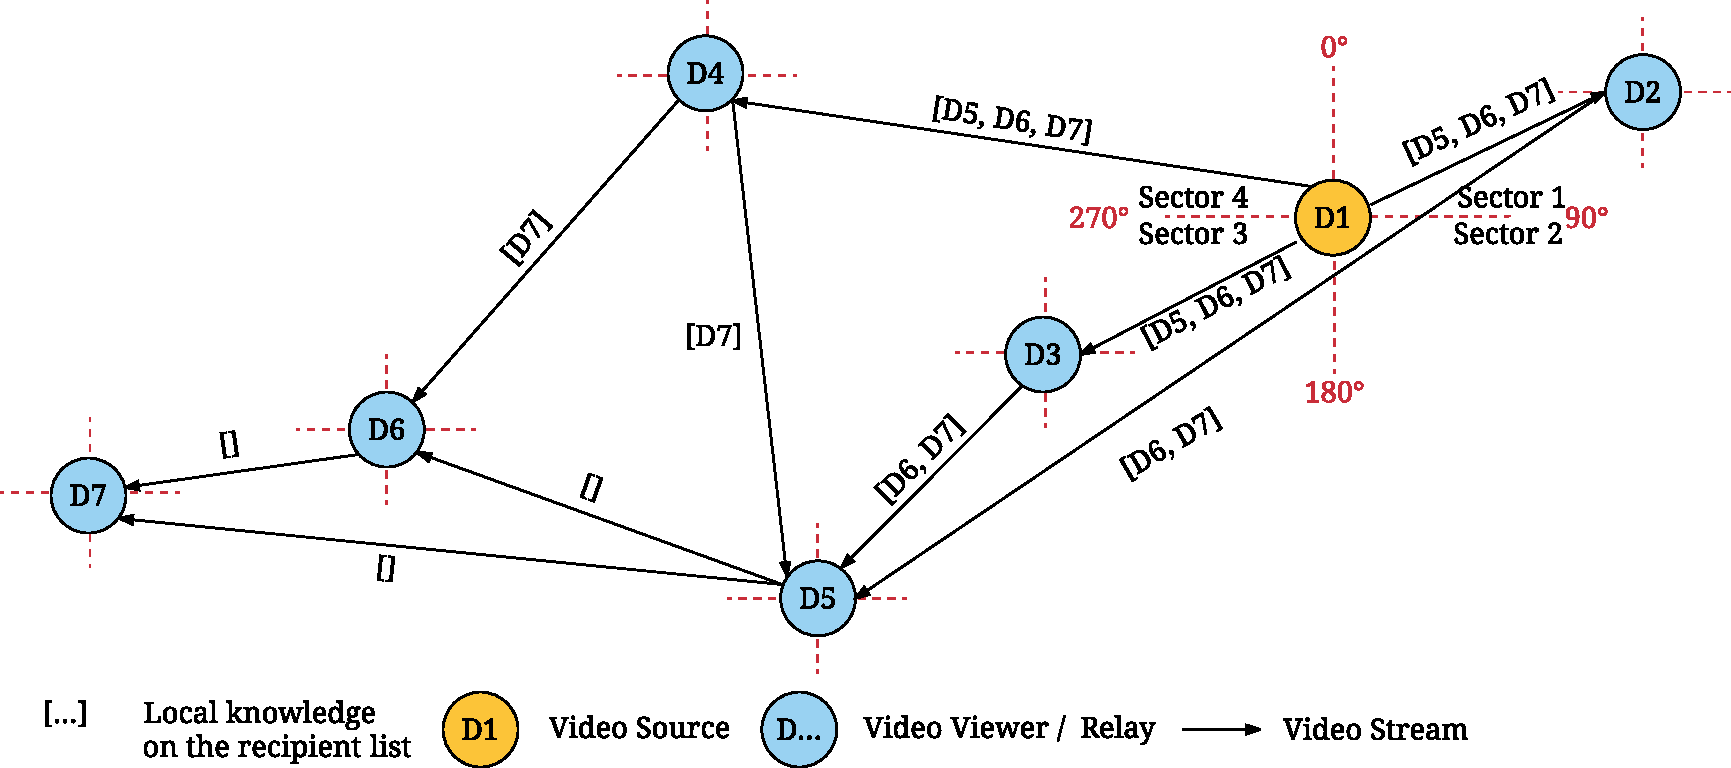
\includegraphics[width=\linewidth]{gfx/500_MobileUpload/MBS_Insitu_Routing_1}
	\caption[Example for LiViU in situ routing of media chunks]{Example for LiViU in situ routing of media chunks in relation to sectors.}
	\label{fig:524_routing1}
\end{figure}

A join message for in situ streaming contains the sender's contact addresses as well as the geographic location of the device. 
To balance the load, a recorder does not directly deliver video streams to all interested receivers, instead it attempts to build a geographically distributed delivery tree. 
Figure~\ref{fig:524_routing1} depicts a typical in situ streaming scenario using \ac{LiViU}.
The recorder determines the relative bearing in degrees ($0\degree$, $360\degree$] and the distance to each interested receiver and relay it knows. 
The bearing indicates the orientation difference to the geographic north; between $0\degree$ and $360\degree$ is divided into sectors of equal size.
Categorizing neighboring devices in an ad-hoc network according to their geo-location is a well-established method, e.g., used for decentralized monitoring systems~\cite{Gross2012}.

In the remaining work, four sectors are assumed with a bearing of ($0\degree$, $90\degree$] for sector one, ($90\degree$, $180\degree$] for sector two, ($180\degree$, $270\degree$] for sector three, and ($270\degree$, $360\degree$] for sector four. 

A higher number of sectors increases the potential number of first hop deliveries, and thus offers a reduced average streaming delay.
The reduction of the number reduces the computational load of the single device.
A receiver or relay is selected from each sector based on the closest distance. 
Each video chunk is distributed to the individual sectors.
A message contains a list of the intended receivers - the so-called recipient list.
Upon receiving a message, the receiver annotates the message and forwards it in a similar manner as the recorder, i.e., selecting the closest recipient in each sector.
If a receiver knows that interested devices are not listed in the recipient list, it adds them.
\begin{figure}
	\centering
	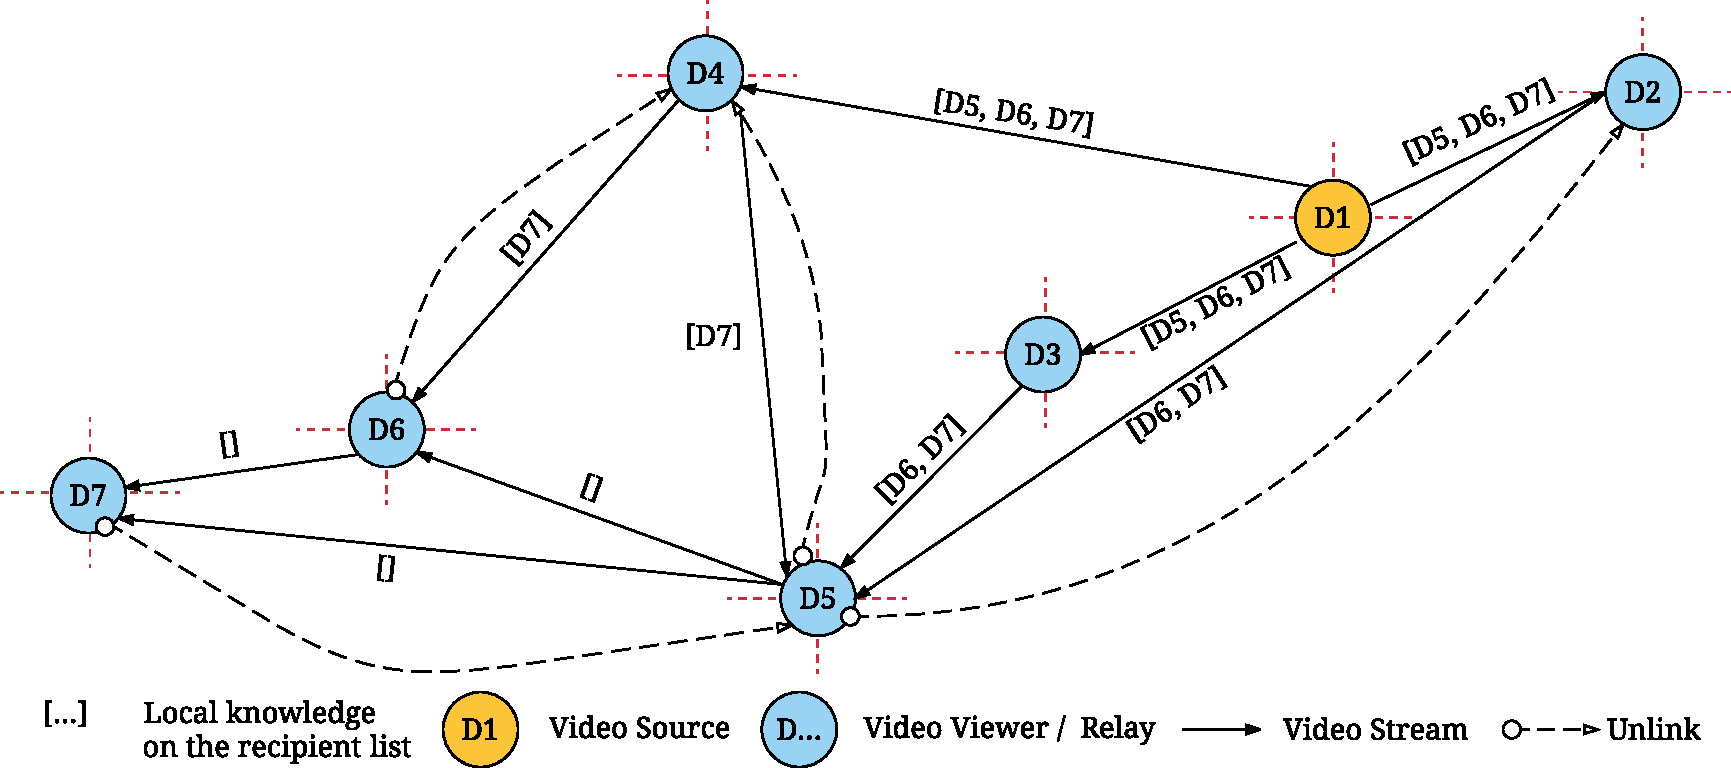
\includegraphics[width=\linewidth]{gfx/500_MobileUpload/MBS_Insitu_Routing_2}
	\caption[In situ routing scheme of LiViU when using unlink messages]{In situ routing scheme of LiViU when using unlink messages to reduce the message overhead.}
	\label{fig:524_routing2}
\end{figure}

Position updates, and thus a recalculation of the distribution topology, are initiated with regularly sent advertisement messages.
Each device advertises at least its position and the unique video stream identifier it is interested.
Also, the advertisement signals a device's online state to all receivers. 
When an interested node no longer wants to receive the stream, it sends an unlink message to the relay node (see Section~\ref{sec:534_unlinking}). 
\subsubsection{Example for Routing Media}
Figure~\ref{fig:524_routing2} illustrates the video dissemination strategy in a second example scenario.
Perfect localization of the devices is assumed, but an imperfection will not significantly harm performance. 
The devices are represented as $D_0$ representing the recorder and $D_1$, $D_2$, $D_3$, $D_4$ and $D_5$ as devices consuming the video stream.
Again, the sector with a bearing of (90, 180] does not contain any interested device and is not considered in the remaining discussion of the example.

A video stream is sent to a first hop from $D_1$ to $D_2$, $D_3$ and $D_4$.
Upon receiving and processing, the recipient list solely contains the remaining devices [$D_5$, $D_6$, $D_7$].
In a next step, the device $D_2$ forwards the video streams to $D_5$ in sector (180\degree, 270\degree], where the remaining sectors are skipped. 
The device $D_2$ forwards the video streams to the recipients in the list: [$D_6$, $D_7$]. 
$D_5$ is omitted as it has received the video from $D_3$.
The device $D_3$ furthermore processes the recipient map [$D_6$, $D_7$]. 
At the same time, $D_4$ forwards a chunk to $D_5$ and $D_6$ with the recipient list solely containing [$D_7$]. 

Thus, the device $D_5$ receives three copies of the same chunk at times $t_1$, $t_2$ and $t_3$. 
It is assumed that $t_1 < t_2 < t_3$. 
When a video chunk is received at $t_1$ from $D_4$, it is forwarded to $D_7$ with an empty recipient list. 
At $t_2$, when a chunk is received from $D_3$, it is forwarded to $D_6$ with an empty recipient list. 
As $D_6$ is closer, the chunk is forwarded only to $D_7$, as the distance is smaller. 
Finally, at $t_3$, when a chunk is received by $D_2$, it is not forwarded at all. 
\subsubsection{Linking and Unlinking Devices}
\label{sec:534_unlinking}
The sector routing prevents unnecessary, redundant routing of video streams to a receiver. 
Due to imprecise positioning data and the design of the routing, mobility situations can occur when a device receives redundant video chunks from multiple senders.

In such a scenario, the push-based delivery of single devices can be stopped by sending an unlink message. 
The unlink message, if received, stops any further relaying of incoming video chunks to the sender of the unlink message.
On the other hand, the link message allows a device to initiate a new stream from a relay, which receives the stream it wants to decode.
The link message acts similarly to a join message, but is instead directed to a relay.
Link messages are used if a device runs out of video chunks in the playback buffer.
As a result, it is possible that a device temporarily receives chunks from multiple devices.
\subsubsection{Reasons for a new Routing Protocol}
Different research groups have proposed routing protocols for ad-hoc streaming.
This paragraph describes why \ac{LiViU} proposes a new approach instead of using protocols such as \ac{AODV}~\cite{aodv} or \ac{OLSR}~\cite{olsr}.
As major \acp{OS} for mobile devices, Android and iOS, have no native support for ad-hoc routing protocols, none of the routing protocols can be run on the lower layers.
Any ad-hoc routing protocol has to be implemented and executed on the application layer.
Thus, a potential efficiency increase in comparison to \ac{LiViU} by running the routing on lower layers is not given.

Also, \ac{LiViU} aims to support in situ streaming, which implies that the devices may be out of communication range but still in the vicinity of a recording device.
In situ streaming implies that the receivers of a stream are on the same event space.
Whereas ad-hoc networks have to cope with large multi-hop scenarios, \ac{LiViU} copes with one or two hops.
One implication is that for a small number of hops a timely propagation of routing information to all devices is possible.
The efficient propagation of routing information across multiple hops is a central goal of ad-hoc protocols.
\ac{LiViU}'s routing protocol is light-weight as each device routes messages without any consultation of other nodes.

As \ac{LiViU} distributes live video streams, data is sent continuously. 
It is very likely that a route is used often in a short time, but the proactive establishment of static routes is infeasible due to device mobility.
\ac{LiViU} acts reactively for the video chunks that are transmitted but leverages geo-location information for the routing.
In contrast to other reactive protocols such as \ac{AODV}, no unnecessary coordination overhead by flooding the devices route request messages occurs, and the route finding time is minimized.

One key attribute of \ac{LiViU} for in situ streaming is risking redundant delivery for the sake of a quick distribution of recorded video chunks.
This is contrary to \ac{OLSR} which informs neighbors on the next hop in order to avoid redundancy.
In contrast, for \ac{LiViU} the receiver of a redundant chunk "unlinks" from its sender to reduce unnecessary data traffic. 
A video stream's source has not to care about the intermediate hops but only about sending a recorded video chunk to the closest receiver in each sector.
Also, more sophisticated routing protocols in ad-hoc networks such as \ac{B.A.T.M.A.N.}~\cite{batmanDraft} do not promise a reduced streaming delay in comparison to \ac{LiViU}.

For \ac{LiViU} only devices that are interested in a video stream participate in the network.
Thus, no complex coordination is required to motivate devices to participate in the ad-hoc network.

Another feature of \ac{LiViU} is that each device can set the number of sectors it supports individually.
We thereby aim that each device can limit the computational load to its capabilities.
The playback and routing of a 1 $\frac{MBit}{s}$ video stream can cause a 100\% CPU utilization on smart mobile devices~\cite{Halvorsen2008}. 
Thus, we avoid to implement one of the protocols and propose with \ac{LiViU} a protocol for efficient low-delay in situ streaming.

The usage of a broadcast of media chunks is avoided, as strong limitations exist in practice. 
The smart mobile devices used during the design, implementation and evaluation phase of \ac{LiViU} limit broadcast transmission to 1 $\frac{MBit}{s}$.
Even with recent video encoding standards, high-quality videos have a higher bit rate~\cite{Sullivan2012}.
\subsection{Message Modifications}
In comparison to the previously mentioned scenario of remote stream receivers, the in situ streaming scenario is based on communication with multiple receivers.
This results in additional coordination overhead, which is required as the routing of video streams addresses multiple receivers, and the devices can be on the move.
The previous sections have illustrated the concepts of allowing \ac{LiViU} to stream in situ.
The remaining section discusses the required message modifications for enabling the in situ communication.
\subsubsection{Header Modifications}
As a result, all messages contain a source field that contains the recorder address.
The source field in comparison to the sender address depicts the origin of a video stream, whereas the sender is different if a receiver retrieves the video from a relay.
\subsubsection{Ad-hoc Messages}
All devices keep local knowledge on their neighboring devices. 
The neighborhood is defined as all devices in communication range.
\paragraph{Advertisement Message}
To know which devices belong to the neighborhood, an advertisement message is periodically sent every $T_{BC,A}= 5$ seconds.
It contains the role of the device and the identifier of the stream, which is currently recorded or received.
The advertisement is sent by each device via broadcast.
It allows retrieving which device is active, providing or consuming video.
\paragraph{Link and Unlink Messages}
Two additional messages are required for the coordination of \ac{LiViU} devices: the link and unlink messages.
These messages are sent to indicate that a device shall start or stop relaying a video stream to the requesting device.
The message is acknowledged by the receiver to indicate to a device that no upload capacity is left.
Unlink messages are used to reduce redundant delivery of messages. 
\section{Supporting different Scenarios}
The combination of mechanisms for remote and in situ streaming allows \ac{LiViU} to support multiple scenarios.
It is assumed that the smart mobile devices support cellular networks and \ac{WLAN} in parallel.
The remote streaming is using the cellular network, whereas the in situ communication is realized using the \ac{WLAN}.
From a recording device perspective, the contact management module allows to distinguish which contact is remote and which is reachable in ad-hoc communication.
As a result, \ac{LiViU} supports hybrid streaming scenarios in real deployments, if two network interfaces can be used in parallel.